


\section{Introduction}
Dynamic PET has been traditionally utilised in single organ studies, but recently there has been increased interest in whole body dynamic imaging, for research and for potential future clinical applications~\cite{Lammertsma2017,Leahy2018,Rahmim2019,Fahrni2019}. Synchronous dynamic PET of the whole body requires scanner geometries that can encompass the entire length of the human body. Although systems capable of whole body axial coverage have been recently developed~\cite{Cherry2017}, their availability is not yet widespread. Current clinical scanners achieve whole body coverage using multiple axial bed positions or acquisition protocols with continuous axial bed motion. Based on these acquisition modes whole body dynamic protocols have been developed that make use of repeated whole body passes~\cite{Karakatsanis2013}. 
Conventional analysis of dynamic data is performed with independent 3D reconstructions of frame data, followed by kinetic model fitting. Whole-body dynamic protocols make the task of reconstruction and subsequent kinetic modelling more challenging due to the introduction of large temporal gaps in the data which can lead to biased estimates and increased noise, especially for parametric maps. 
To improve image quality and account for the noise in the raw data, 4D reconstruction algorithms can be used to directly incorporate the dynamic model of interest in the reconstruction~\cite{Reader2014}.
Depending on the choice of the dynamic model, these reconstructions can directly provide the parameters of interest or temporal regularisation on the reconstruction process of frame data. The spectral analysis model, inspired by the homonym method~\cite{Cunningham1993}, fits on any underlying kinetic behaviour that can be described by compartmental modelling. When used in 4D reconstruction it provides temporal regularisation as well as direct estimation of some kinetic parameters. Use of this model has shown to reduce noise and bias of kinetic parameter estimates when applied on data from whole body dynamic protocols~\cite{Chalampalakis2019}.

When considering the effective field of view of whole body dynamic studies, certain regions might not fulfil the generic assumptions of the spectral analysis model. For example processes such as delay of tracer delivery and non-arterial tracer delivery (ex. bladder filling).
In 4D reconstruction, the tomographic update process is entangled with the dynamic model and errors from the temporal model fit have the potential to spatially propagate to other regions. Due to the fact that raw data from multi-bed whole body dynamic studies are acquired and reconstructed as separate beds, the potential for errors propagation is limited in the bed position where they originate from. It has also been shown that use of time of flight (TOF) information in the reconstruction aids in reducing spatial propagation of errors~\cite{Kotasidis2016a}. Nevertheless, model fit errors have the potential to propagate and when possible should be corrected or accounted for. For this reason, when 4D reconstruction is used and especially when applied on whole body datasets extra consideration has to be given on improving the model fit for all regions.

The application of an adaptive residual model as a second dynamic model has been previously suggested for reducing model fit errors~\cite{Matthews2012}. Its application in 4D reconstruction has been shown to reduce bias at the cost of increased noise for direct estimation of kinetic micro-parameters~\cite{Kotasidis2014c}.
The objective of this work was to implement and evaluate adaptive residual modelling in 4D reconstruction, using real whole body dynamic PET data, with no prior knowledge of the underlying kinetics and the distribution of residuals. For this purpose, the spectral analysis model was used in conjunction with a residual model in 4D reconstruction to maintain genericity in the reconstruction with minimum assumptions on the underlying kinetics. 
The end objective was to assess if adaptive residual modelling can be permanently applied in 4D reconstruction, with no prior knowledge of kinetics and model fit errors, by relying on the selectivity of the algorithm for correction of underlying model fit errors, when and where those arise. 
%-------------------------------------------------------------------------------

\section{Methods}
\subsection{Data acquisition}
Dynamic whole body data using a novel Glyburide (${}^{11}C$-GLB) tracer were acquired from healthy volunteers on a GE Signa PET-MR, using a dedicated dynamic protocol of 5 bed positions to provide sufficient coverage of the body. Glyburide is a substrate of hepatic and extrahepatic Organic Anion Transporting Polypeptides (OATP) which can be isotopically radiolabelled with carbon-11 for PET imaging. The data were acquired as part of the exploratory pharmacokinetic study IsotoPK which is conducted in our centre for studying the distribution of OATP transporters in the body and their role in the delivery of drugs to tissues~\cite{Marie2019}. 
Data from a single volunteer study were used in this work. In detail the dynamic acquisition consisted of a single bed acquisition centred over the liver, imaged for 3 minutes from tracer injection, followed by 14 whole body passes of 9x20s and 5x30s frames for each bed position. 
Arterial blood samples were collected manually during the whole study, to measure the input function.
\subsection{Reconstruction}
The spectral analysis model was used in all 4D reconstructions, using 4 spectral functions with decay rates ranging from 3 \(min^{-1}\) to 0.001 \(min^{-1}\). A constant and a delta function were also included to model tracer trapping and blood fraction. The 4D reconstruction algorithm with adaptive residual modelling was developed using the spectral model as primary model and an adaptive secondary model, similar to the proposed method by Matthews et al.~\cite{Matthews2012}. 
 
The steps of the adaptive residual modelling 4D reconstruction algorithm are:

\begin{enumerate}
  \item Start with image estimate $\lambda_{jf}^{(k)}$, for voxel $j$ and frame $f$ at iteration $k$. 
  \item Perform tomographic update using MLEM to get the EM update image $\lambda_{jf}^{(EM)}$.
  \item Perform primary model fit using the NNLS algorithm on $\lambda_{jf}^{(EM)}$ and estimate model parameters $\bm{\theta}_{j}^{(k+1)}$.
  \item Calculate residuals as $ r_{jf} = \lambda_{jf}^{(EM)} - f_{spectral}(\bm{\theta}_{j}^{(k+1)}) $.
  \item Perform PCA analysis on residuals to estimate a set of residual basis functions (RBF) which form the secondary (adaptive) model. 
  \item Estimate modelled residuals $g_{jf}$ from the LS fit of the secondary model on the $r_{jf}$ data. 
  \item Estimate optimal fraction $K_{j}$ for residuals re-introduction, using generalised cross validation.
  \item Add fraction of modelled residuals in image estimate $\lambda_{jf}^{(k+1)} = f_{spectral}(\bm{\theta}_{j}^{(k+1)}) + K_{j} g_{jf} $ and repeat from step 2.
\end{enumerate}

where NNLS stands for Non-Negative Least Squares and $f_{spectral}$ is the spectral model which provides activity distribution maps for all frames, given model parameters $\bm{\theta}_{j}$. 
        
In step (5) of our adaptive modelling implementation, the residual data were spatially smoothed with an isotropic Gaussian kernel of 32mm FWHM, to enhance the PCA analysis results. Smoothing of the residuals was not however applied in the fitting process of the secondary model in step (6). A fixed number of the most significant PCA components was used as basis functions of the adaptive residual model. The components were updated on each iteration of the 4D algorithm.

For the estimation of the optimal fraction $K_{j}$, the following equation from Matthews \textit{et al.}~\cite{Matthews2012} was used, which is derived from generalised cross-validation,

\begin{equation}
K_{j} = \frac{1-\frac{r_{df}}{r_{RSS}}}{1-r_{df}} , 
\end{equation}

where $r_{df} = \frac{n_s}{n_f - n_p}$, with $n_p$ and $n_s$ being the number of parameters of the primary and secondary model respectively, and $r_{RSS}$ being the fraction of modelled to measured residuals sum of squares. 

% with the $r_{df}$ ratio of degrees of freedom of the residual model to residual space being  0.375(0.25).

The dynamic data from each bed of the study were reconstructed as individual frames using 3D MLEM (150it), using 4D reconstruction (300it) and with the developed adaptive algorithm 4D-ResidMod (300it). The adaptive reconstruction algorithm was evaluated using the 2 and 3 most significant PCA components as RBFs, referred to as 4D-ResidMod-2RBF and 4D-ResidMod-3RBF respectively. We also implemented a version of the adaptive algorithm with the addition of temporal Gaussian smoothing of 62s FWHM applied on the residual data used for PCA analysis in step (5) of the algorithm, referred as reconstruction 4D-ResidMod-3RBF-Tempfilt.

All reconstructions were performed with the open source reconstruction platform CASToR~\cite{Merlin2018}, using PSF modelling and TOF information. Correction for motion has not been included in the reconstructions. PCA analysis was performed using the Eigen library~\cite{eigenweb}. 
%------------------------------------------------------------------------------

\section{Results}
As seen in Fig.~\ref{fig:Frame14Differences} (top row) by the difference in activity estimates from 3D and 4D reconstruction in a late frame, the 4D algorithm with the spectral model alone resulted in lower activity estimates over the bladder region and higher activity estimates in some large blood vessels at the shoulders and pelvic regions. No noticeable differences were seen in other areas, apart from random variations in activity due to differences in noise levels of the compared reconstructions.
As expected, the filling process of the bladder seen in the bladder time activity curve from 3D reconstruction in Fig.~\ref{fig:TACs} (bottom row) cannot be modelled by the spectral model because the filling process is not directly relatable to arterial tracer delivery at the local (voxel) level. Differences in some large blood vessels could potentially be attributed to delay of the input function, which is not accounted for in the spectral model where a single input function is assumed to apply for all regions. 

Reconstruction of the data with adaptive residual modelling resulted in improved estimation of the bladder filling process, for both options of residual modelling using 2 and 3 residual basis, as it can be seen in the difference images of Fig.~\ref{fig:Frame14Differences} (middle row) and the bladder TAC in Fig.~\ref{fig:TACs}. 
No improvements were seen for the differences at the blood vessels of the shoulders and pelvic regions. 

At the liver, where most of the tracer uptake is concentrated, 4D and 3D reconstruction TACs show a subtle mismatch between 1100 and 1500 seconds (Fig.~\ref{fig:TACs}, top row). Analysis on the liver dome VOI (Fig.~\ref{fig:TACsFilt}, top row) clearly shows this difference, which originates from underlying respiratory motion that has been captured in the PET dynamic data. 4D reconstruction alone was unable to model these fluctuations, as expected, but the adaptive algorithm using 3 residual basis has achieved to model for this behaviour as seen in Fig.~\ref{fig:TACsFilt}.
Since physiological kinetic processes, whether sufficiently modelled or not, are not expected to result in sudden changes of activity between adjacent frames, we implemented a version of the algorithm with temporal smoothing prior to PCA analysis to prevent from modelling changes due to fast processes such as respiratory motion. On this case this algorithm (4D-ResidMod-3RBF-Tempfilt) has managed to maintain the selective adaptive modelling behaviour over the bladder while avoiding fitting the motion related effects over the liver dome as seen in Fig.~\ref{fig:TACsFilt}. 

\begin{figure} [h!]
\centering
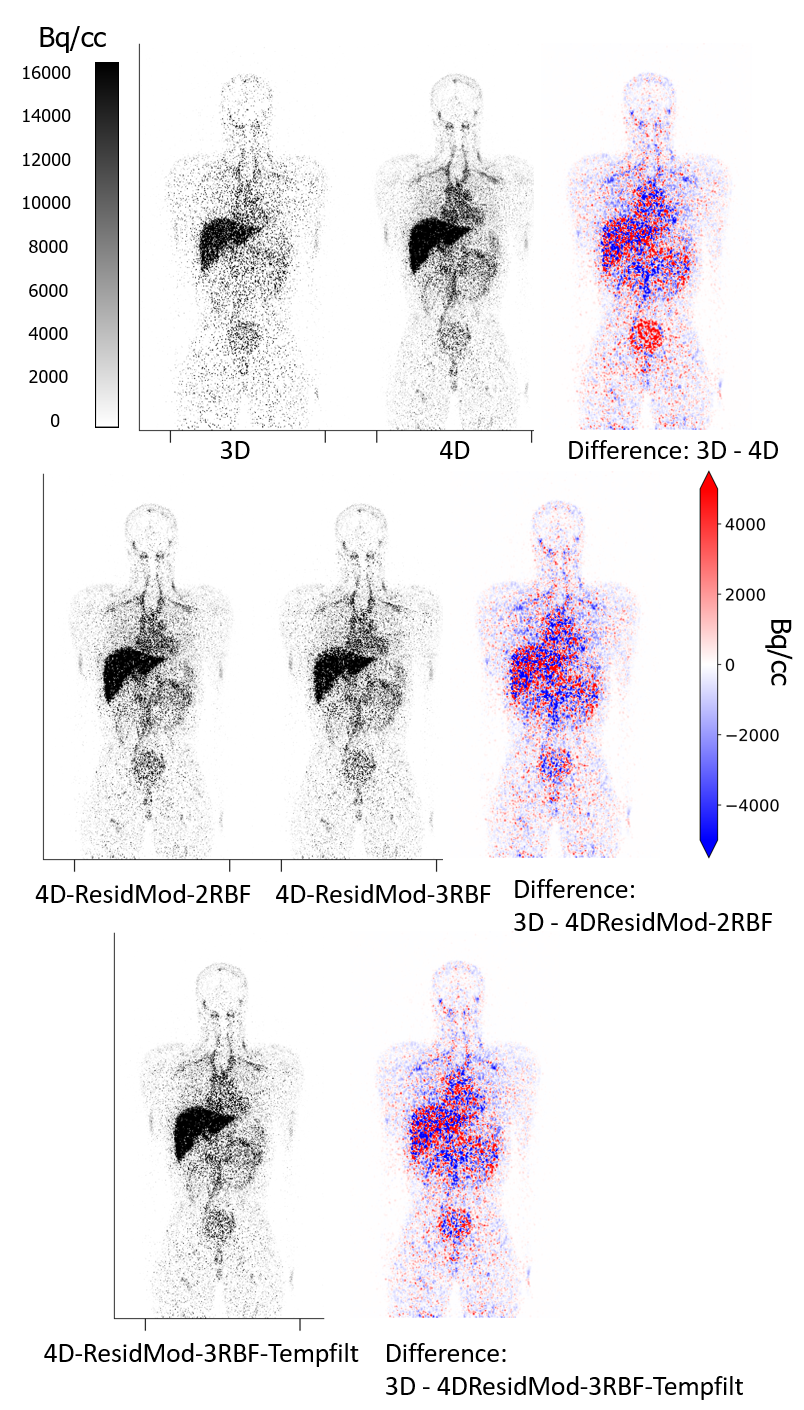
\includegraphics[scale=1.25, angle=0]{3_Results/3_4_Residual/figures/Frame14DifferencesV2.png}
\caption{Coronal view of activity distribution from the evaluated reconstructions (frames of 41.2 to 44.1 minutes post injection). Difference images are also shown for selected cases against the 3D reconstruction.}
\label{fig:Frame14Differences}
\end{figure}

\begin{figure} [h!]
\centering
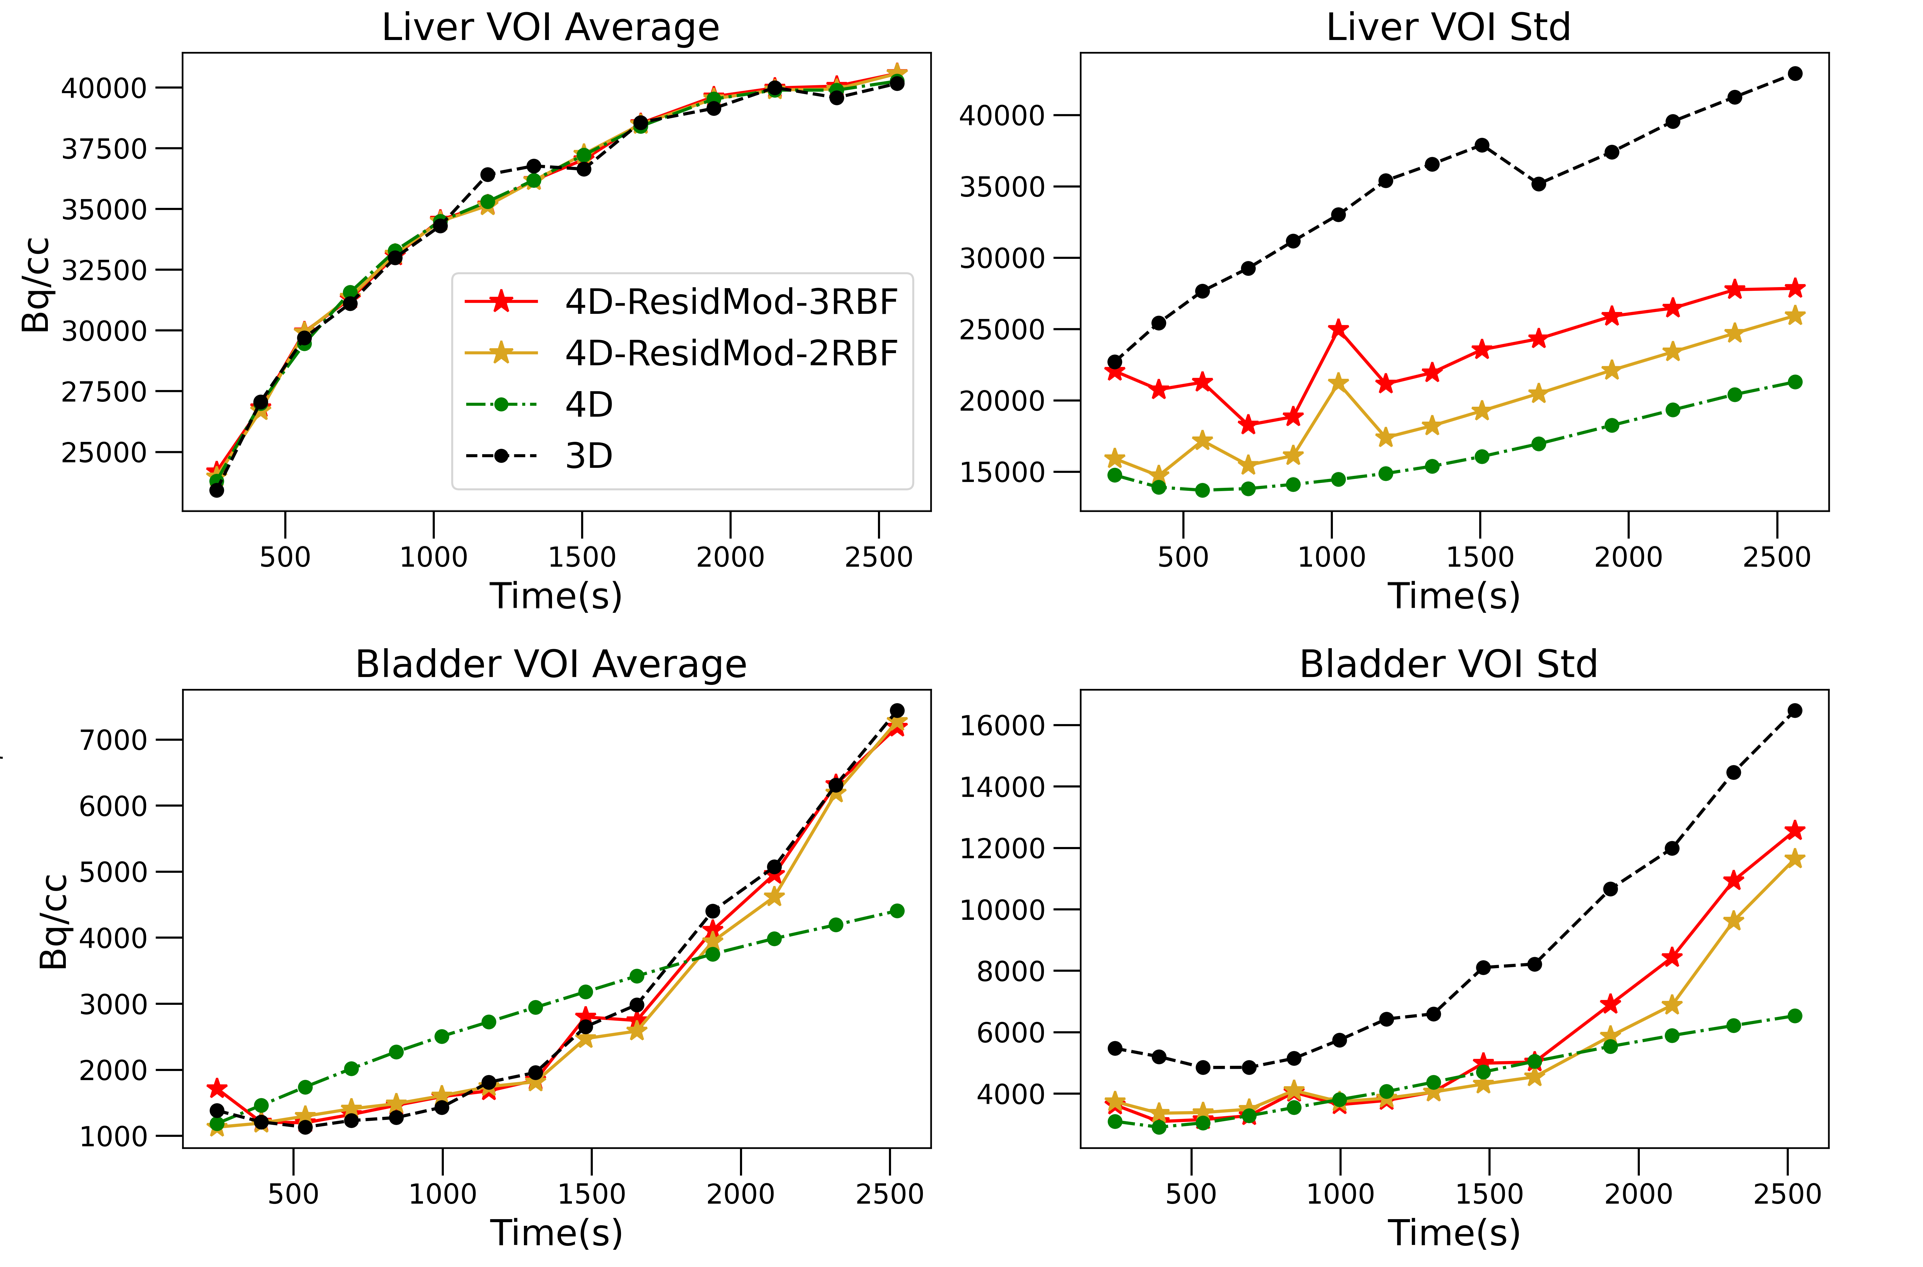
\includegraphics[scale=0.64,angle=0]{3_Results/3_4_Residual/figures/TACs.png}
\caption{Average and standard deviation time curves of the liver and bladder VOIs, for the comparison of 3D to 4D reconstruction results as well as 4D reconstruction with residual modeling using different number of residual basis functions.} 
\label{fig:TACs}
\end{figure}

\begin{figure} [h!]
\centering
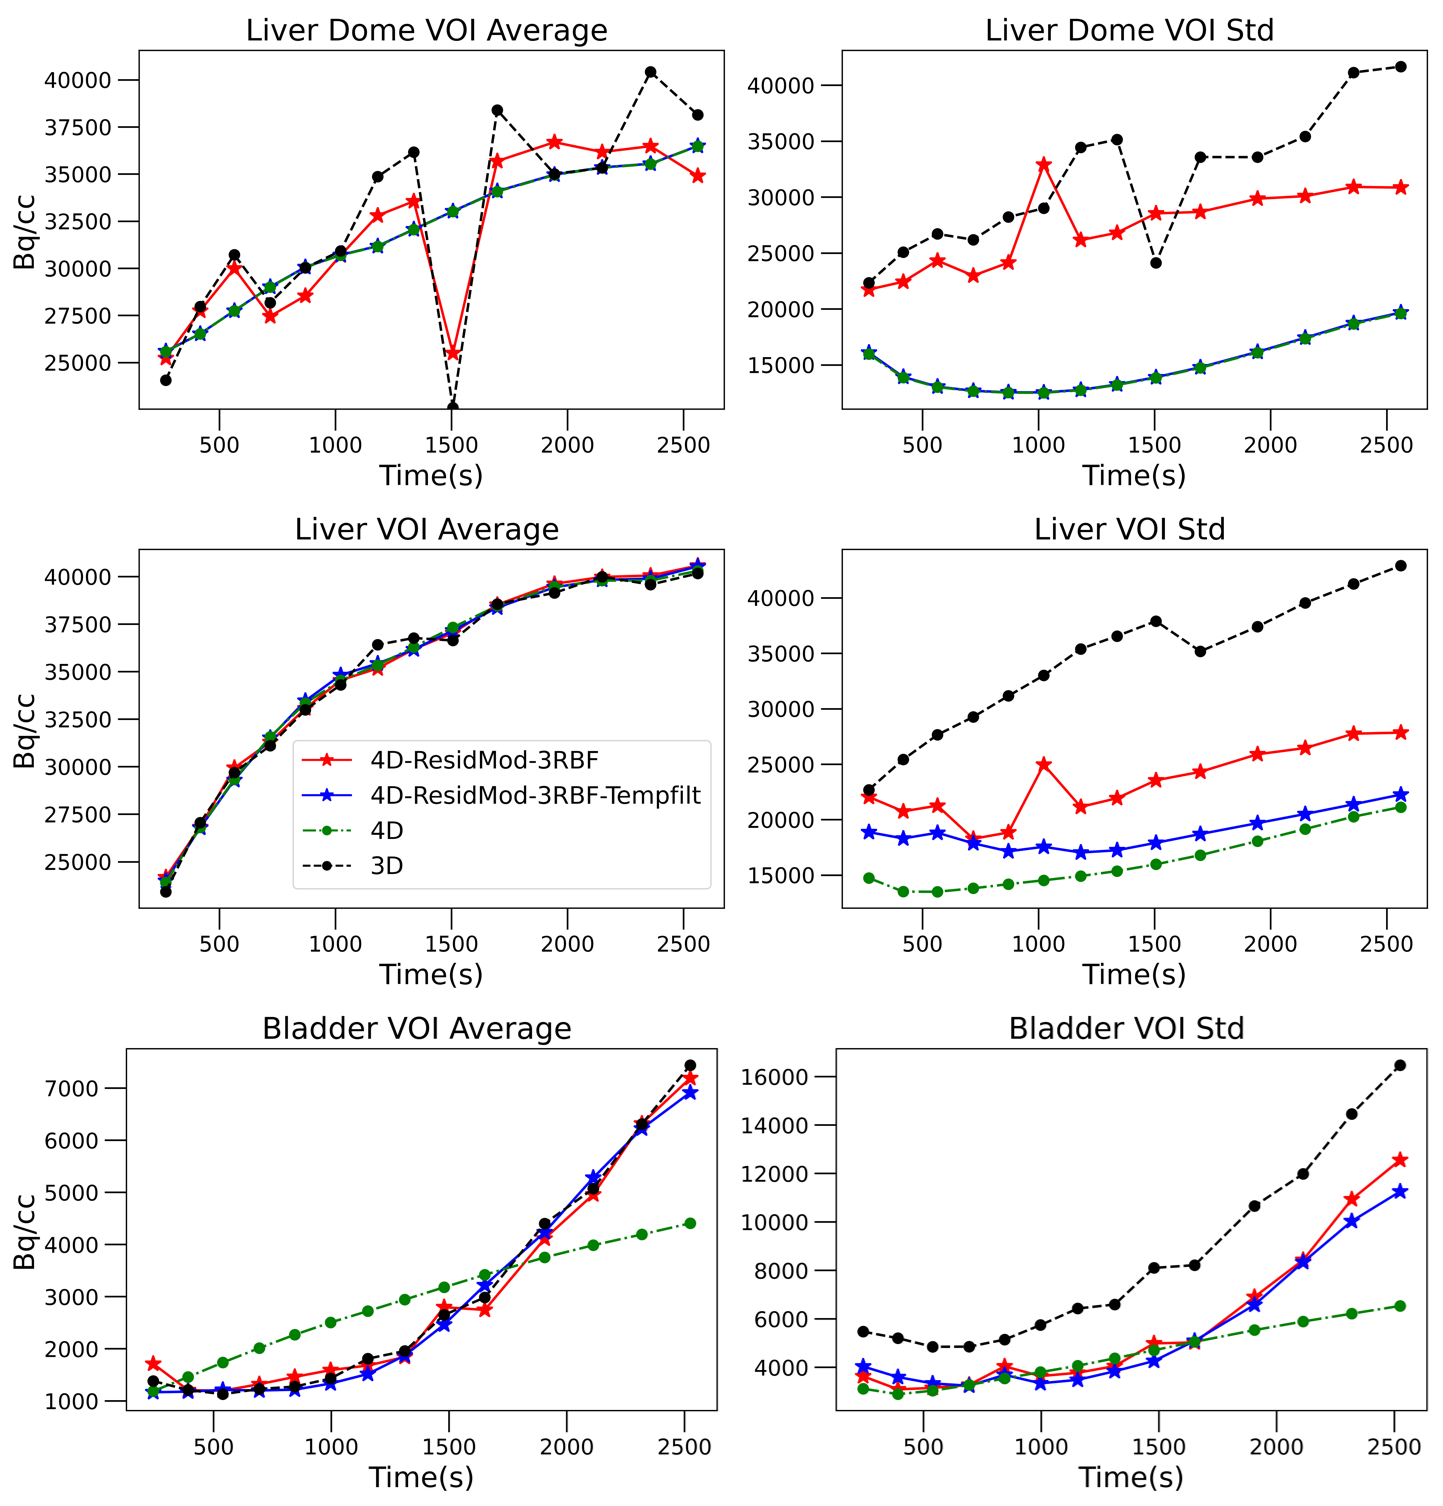
\includegraphics[scale=0.74 ,angle=0]{3_Results/3_4_Residual/figures/TACsFilt.png}
\caption{Average and standard deviation time curves of the dome of the liver the whole liver and bladder VOIs, for the comparison of 4D reconstruction with residual modeling with and without temporal filtering of residuals.} 
\label{fig:TACsFilt}
\end{figure}


In all regions of the effective FOV the addition of adaptive modelling has resulted in the increase of image noise, compared to 4D reconstruction, with the higher number of residual basis resulting in higher noise. The introduction of temporal filtering in the adaptive model estimation process has aided in reducing the induction of noise for the majority of the evaluated regions in our study. 
A comparison of the effect on image noise across regions within this whole body study can be made by the VOIs standard deviation shown in Fig.~\ref{fig:BarPlot} for all evaluated algorithms.
An example map of the fraction $K_{j}$ and the modelled residuals $g_{jf}$ is given in Fig.~\ref{fig:FractionMap}. These maps demonstrate the desired selectivity of the algorithm, concentrated over the bladder in this case, but also the
spill of noise from the residual space in these maps which is subsequently added in the reconstruction process.

\begin{figure} [h!]
\centering
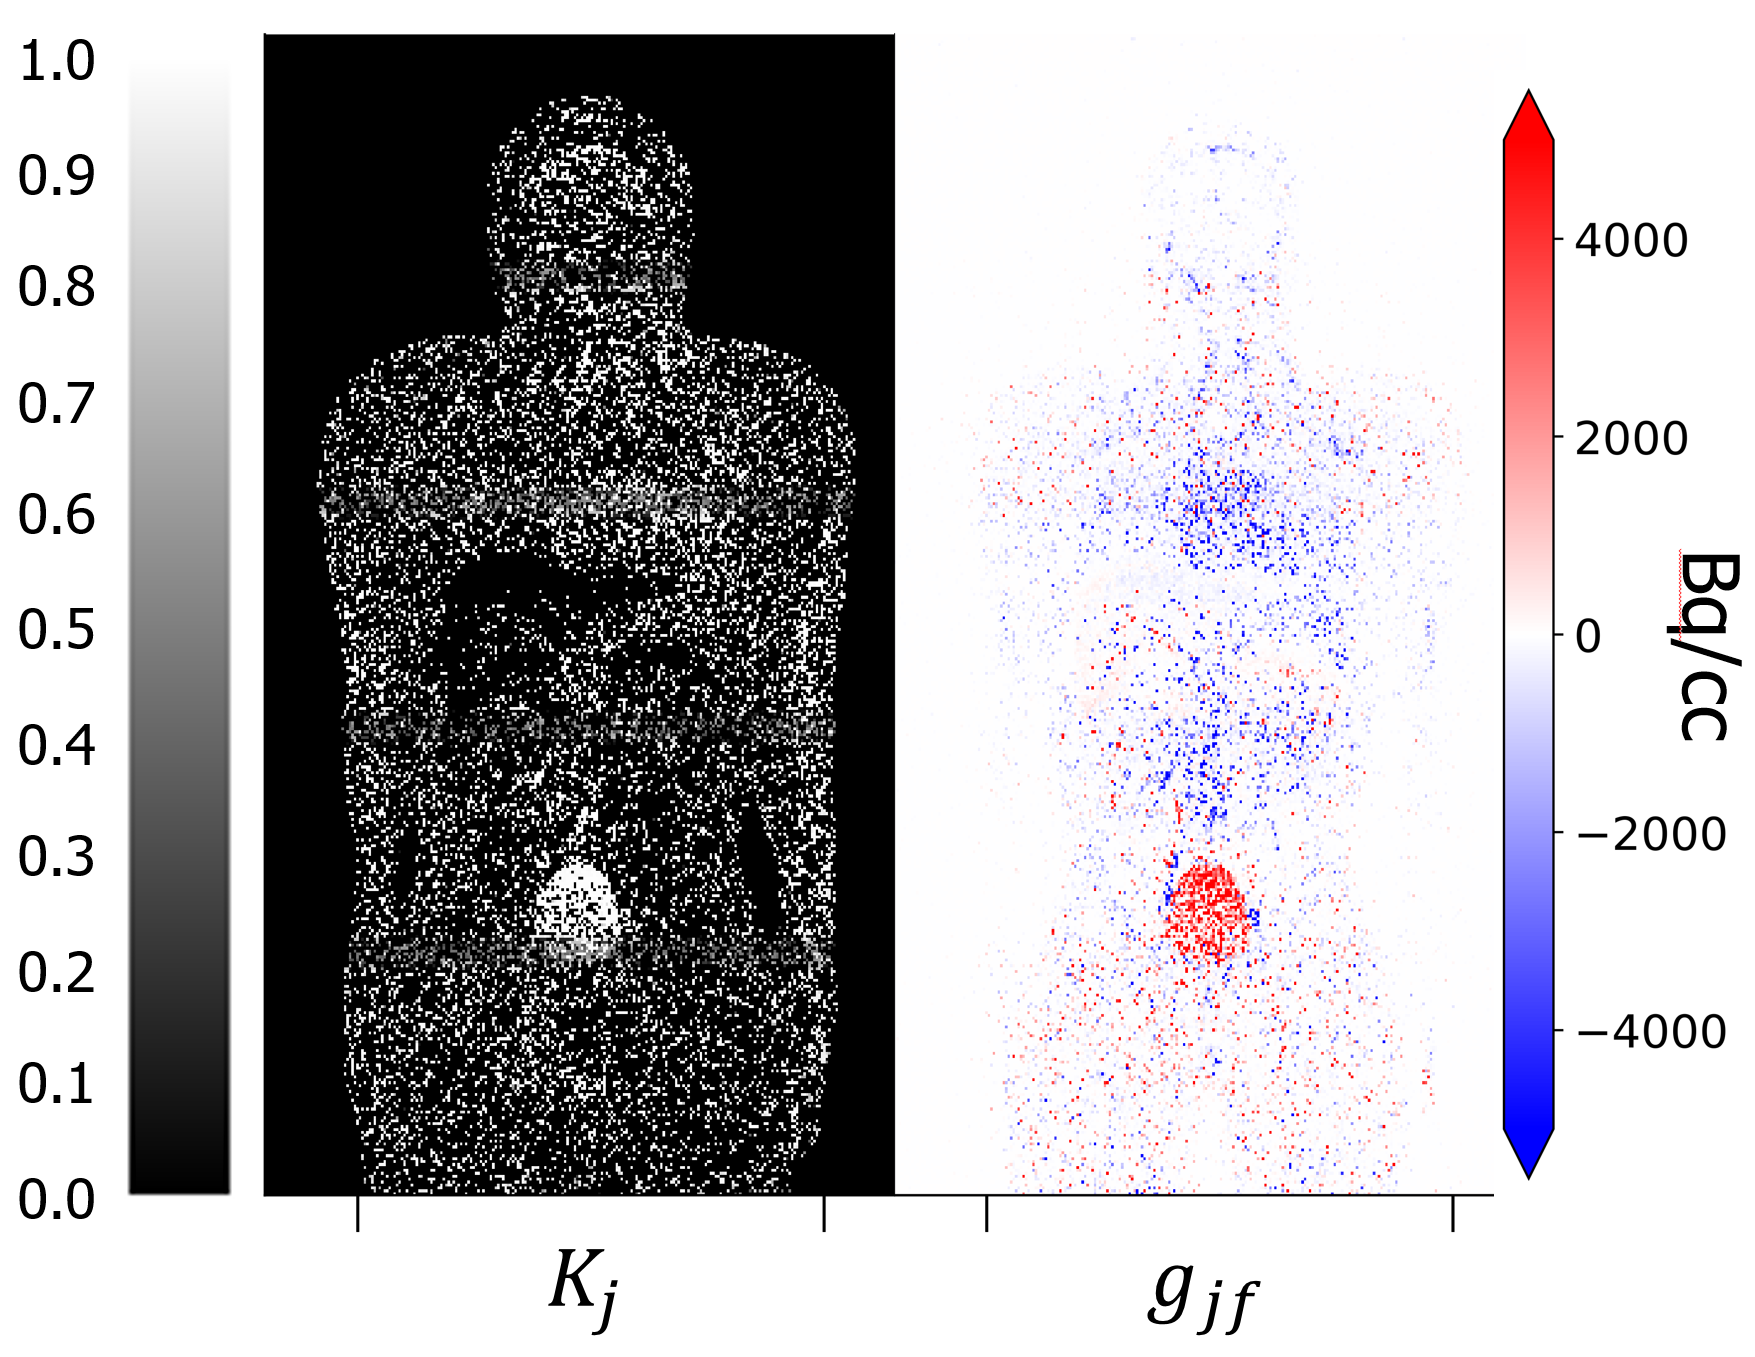
\includegraphics[scale=0.44 ,angle=0]{3_Results/3_4_Residual/figures/FractionMap.png}
\caption{Fraction map of $K_j$ and modelled residuals $g_{jf}$ of the residual model 4D-ResidMod-3RBF-Tempfilt at iteration 75.} 
\label{fig:FractionMap}
\end{figure}

\begin{figure} [h!]
\centering
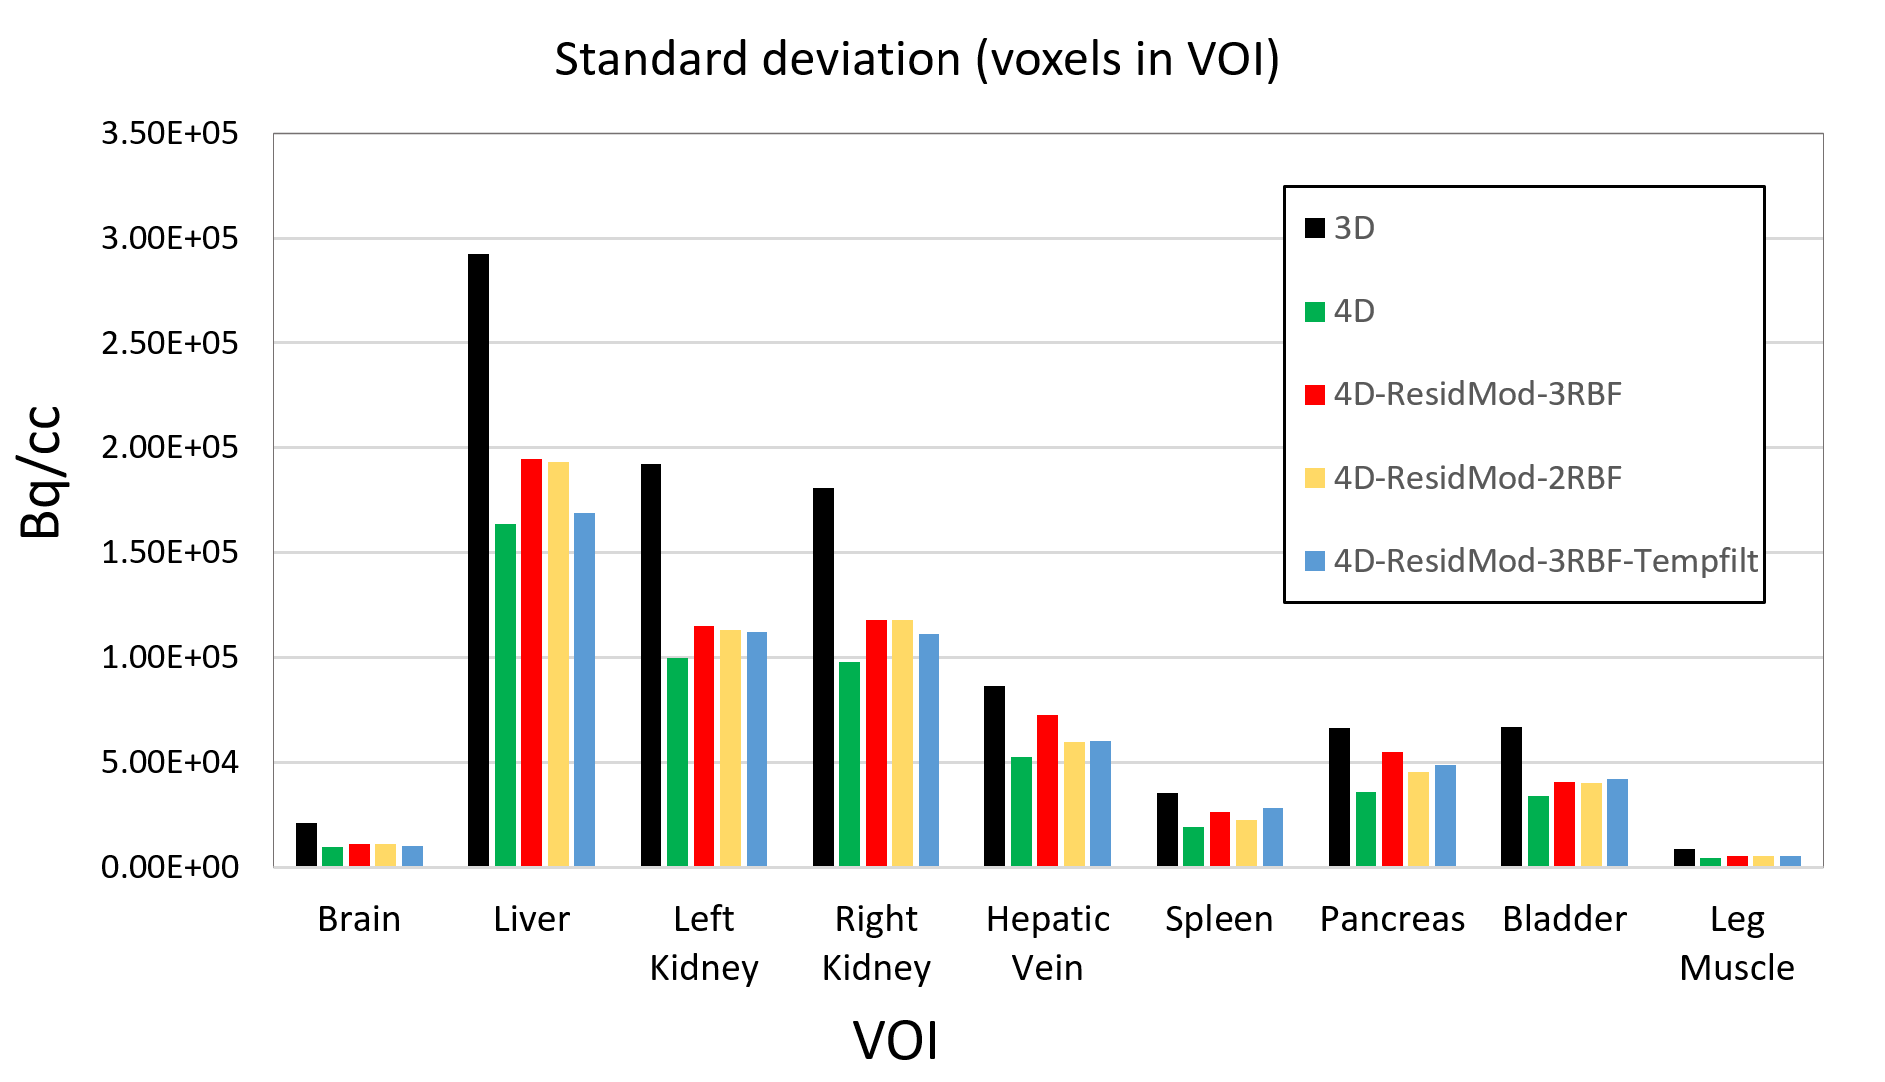
\includegraphics[scale=0.65 ,angle=0]{3_Results/3_4_Residual/figures/BarPlot.png}
\caption{Standard deviation of VOIs for regions in the whole-body, for all evaluated reconstructions.} 
\label{fig:BarPlot}
\end{figure}


\section{Discussion and Conclusion}
General dynamic models such as the spectral analysis model can be useful in 4D reconstruction of whole body dynamic data using new tracers, as they do not impose strong assumptions about the underlying kinetics. But over the effective field of view of whole body dynamic studies certain regions and their physiological processes might not fulfil the general assumptions of the model. In these cases, the adaptive residual modelling strategy can be utilised to improve parameter estimates for these regions and help in minimising the risk of spatial propagation of errors to other well modelled regions.

%Due to the fact that raw data from multi-bed whole body dynamic studies are acquired and reconstructed as separate beds, the potential for errors propagation is limited in the bed position where they originate from. Also it has been shown that use of time of flight (TOF) information in the reconstruction aids in reducing spatial propagation of errors~\cite{Kotasidis2016a}. Nevertheless model fit errors have the potential to propagate and when possible should be corrected or accounted for.

In this work, 4D reconstruction with the spectral analysis model and adaptive residual modelling was applied on real whole body dynamic data from a first in man study of a new tracer. The algorithm identified and selectively corrected the image activity estimates over the poorly modelled bladder region, by modelling the residuals of that region. This resulted in a 4D reconstruction that did not suffer from the model fit errors over the bladder and potential errors propagated to other regions originating from the bladder region. 
The use of the adaptive model as a secondary model increased the complexity of the modelling in the reconstruction process and resulted in an increase of image noise, with higher number of residual basis functions resulting in higher image noise as expected and inline with previous observations in a simulation study~\cite{Kotasidis2014c}.
In our work we saw that noise from the residual space propagates in the modelled residuals and the optimum fraction values of the secondary model, seen in Fig.~\ref{fig:FractionMap}, and is subsequently re-introduced in the reconstruction process. 

Motion will unavoidably always be present in the raw data of dynamic studies and when it is not accounted for in the 4D reconstruction process will give rise to model fit errors. In our evaluation we saw that the adaptive algorithm attempted to model residuals caused by respiratory motion, when the level of complexity of the secondary model permitted that, even though this was not its original intended use.
As any tracer's kinetic processes are expected to be slower than variations due to respiratory motion, pre-treatment of residuals with temporal filtering in the residual model estimation step aided in averting the adaptive model from fitting these motion induced differences while maintaining its capability of modelling kinetic processes. In addition, temporal filtering also aided in reducing the increase in noise from the use of the secondary model.

In this work we conclude that the use of the secondary adaptive model based on PCA analysis can be a practical solution to spectral analysis model fit errors, when added to the generic 4D reconstruction algorithm used with whole body dynamic data from new tracers. The combination of spatial and temporal filtering in the treatment of residual data prior to PCA analysis provided the optimal results in our tests, in terms of algorithm selectivity and levels of added noise. 


%Finally it is expected that the behaviour of the adaptive model will strongly be affected by the nature of the underlying kinetics and the raw data, so the option of its parameters (number of basis, strength of spacial and temporal filtering, iterations of the model) will need to be fine tuned for each study. 
